%===============================================================================
% $Id: ifacconf.tex 19 2011-10-27 09:32:13Z jpuente $  
% Template for IFAC meeting papers
% Copyright (c) 2007-2008 International Federation of Automatic Control
%===============================================================================
\documentclass{ifacconf}

\usepackage{graphicx}      % include this line if your document contains figures
\usepackage{natbib}        % required for bibliography
%===============================================================================
\begin{document}
\begin{frontmatter}

\title{Prediction of Disease Phenotype \& Inference of Gene Networks: Revisting the DREAM5 Systems Genetics Challenge}

\author[First]{Vankiripalli Mohammad Aaftab}
 
\address[First]{Department of Mechanical Engineering, IIT Madras (e-mail: aaftaabv@gmail.com)}



\end{frontmatter}

%===============================================================================

\subsection{First Report}

The DREAM5 Systems Genetics Challenge Part-B consists of 3 parts.In the First part, the problem is to predict the extent of disease phenotype existence based on the Genotype of a particular plant.There are 941 genotype variants in 200 plants (genotype variants represent either the presence or absence of a gene in each of the 200 plants).Hence, the training data for this problem consisted of a 200X941 boolean type matrix and the extent of disease presence in each plant is given as a seperate 200X2 matrix with each plant having 2 different phenotype values both representing the effect a particular pathogen(Phytophthora sojae).Hence we had 200 plants with each plant having 941 features which can be used to predict 2 different phenotype values.So the Machine Learning model took 941 features from each of the 200 plants and fitted a model(seperately) using these features to predict outcomes(phenotype1, phenotype2).

The prediction of phenotype was to be done on a testing set that consisted of 30 plants with variations across 941 genes given.Machine Learning Models were trained on the training set and these models were used to then predict the phenotype values(real numbers) for the 30 plants in the test data set.
The predicted phenotype value was compared with the given gold standard phenotype values using spearman correlation coefficient and p-value. 

Similarly in the second sub-challenge, the training data consisted of a real 200X28,395 matrix of gene expression values and a 200X2 real matrix representing phenotype values in each plant.And the prediction of phenotype had to be done only based on the given gene gene expression values in each plant. Again the models were fit on the training data and predicted on the test dataset that consisted of gene expression values of 28,395 genes in 30 different plants.The predicted phenotype value was compared with the given gold standard phenotype values using spearman correlation coefficient and p-value. 
Here also we had 200 plants with each plant having 28,395 features that can be used to predict 2 different outcomes.So the Machine Learning model took 28,395 features from each of the 200 plants and fitted a model using these features to predict outcomes(phenotype1, phenotype2).

Finally the score of each model was calculated as was done by the DREAM5 Systems Genetic Challenge i.e. sum of natural logarithms of p-values of spearman correlation between given gold standard phenotype values and predicted phenotype values. (There were two predictions in each subchallenge one corresponding to phenotype 1 and the other corressponding to phenotype2 )

The models used for the subchallenge1 include:Linear Regression, Lasso Regression, Decision Tree, Random Forest, SVM,AdaBoost,Bagging Regressor,Gradient Boosting Machine(GBM),Homogeneous Voting Regression(using Random Forest Models and GBM),Cat
-Boost Regressor.

The models used for the subchallenge2 include:Linear Regression, Lasso Regression, ElasticNet regression,Decision Tree, Random Forest, SVM,AdaBoost,Bagging Regressor,Gradient Boosting Machine(GBM),Homogeneous Voting Regression(using Random Forest Models and GBM).

\begin{figure}
\begin{center}
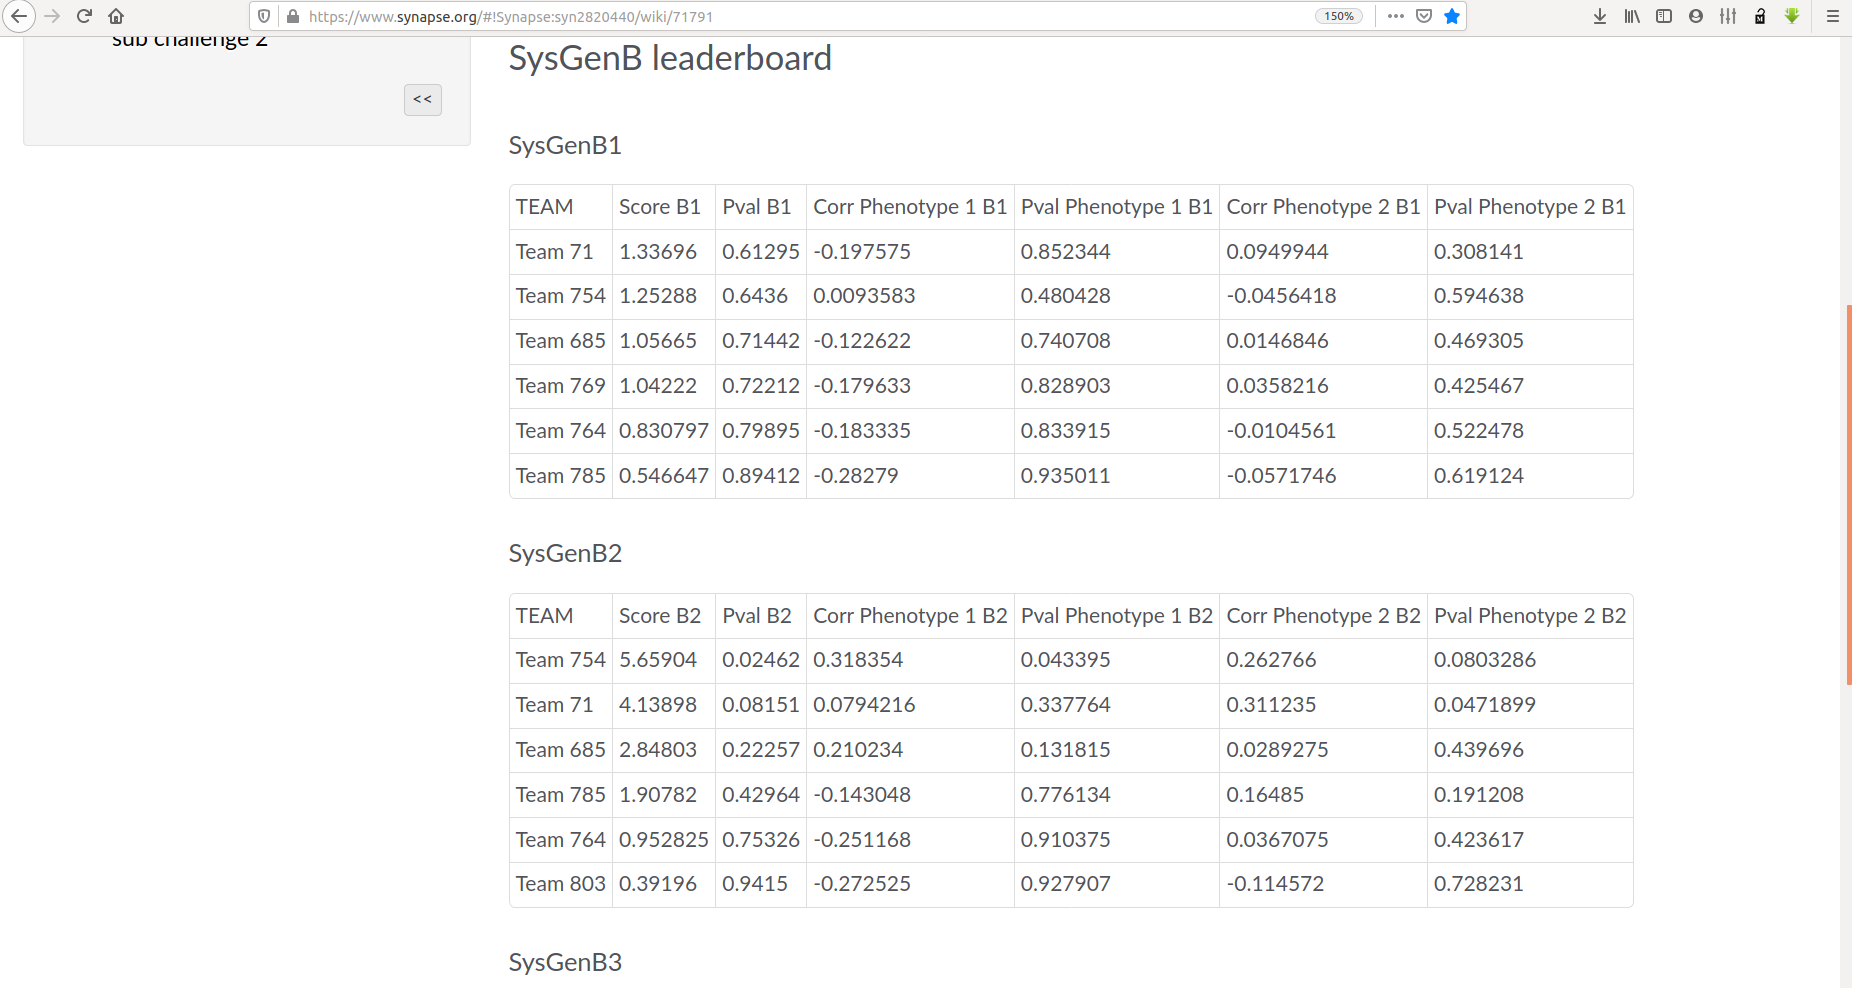
\includegraphics[width=8.4cm]{leaderboard}    % The printed column width is 8.4 cm.
\caption{DREAM5 SysGenB Challenge Leaderboard } 
\label{fig:leaderboard}
\end{center}
\end{figure}

From the above leaderboard, it can be seen that the best score in the challenge B1(i.e. inference of Phenotype only from Genotype data) is 1.33696, whereas my score for Linear Regression is 2.2044070348685127.
Till this point of time, the given data was scaled using standard scaler method in Sklearn and was used to fit a model using various machine learning algorithms. The other ML algorithms that beat the then best score are Ridge Regression, Bagging Regression, GBM regression, Voting Regression using only GBM models, and Catboost Regressor.

I plan make further improvements to the model by using PCA(linear dimensionality reduction), Manifold Learning(Non-linear dimensionality reduction) etc.Right now the number of features is about 941 which might introduce curse of dimensionality to some models.Next step will be to analyse data using dimensionality reduction.

The score was calculated by this procedure:

Spearman correlation coefficient and P-value was found between the real values of phenotype1 and predicted values of phenotype1 and the same 2 values were found between real values of phenotype2 and predicted values of phenotype2.The score is -1*(natural logarithm of p-value of spearman correlation between phenotype1's real and predicted values + natural logarithm of p-value of spearman correlation between phenotype2's real and predicted values).

For the subchallenge B2(i.e. prediction of phenotype based only expression values of 28,395 genes), the best score in the leaderboard is 5.65904. My decision tree regressor model had a score of 6.283454289075021.Other models that surpassed the best score on leaderboard include Random Forest, Gradient Boosting Machine(GBM), GBM voting regressor.

The B2 challenge had an even larger feature space (28,395 features ) than B1 challenge hence we expect the models to perform even better on this data after linaer or non-linear dimensionality reduction is applied.

The score was calculated by the same procedure as indicated above.
The complete scores of each model on SysGenB1 and SysGenB2 is summarised in the below table. 

The following table illustrates the Model vs problem statement information of used models.

\begin{table}[hb]
\begin{center}
\caption{Scores Table}\label{tb:margins}
\begin{tabular}{cccc}
Model & B1 Score & B2 Score  \\\hline
Linear Regression & 2.2044070348685127 & 1.4372172661318754  \\
Ridge Regression & 2.1819492446231603 & 1.4371453159087157  \\
Decision Tree Regression & 0.4965799903304826 & 6.283454289075021 \\ 
Random Forest Regression & 0.45537125620964347 & 5.792798653297446  \\
SVM Regression & 0.6627204323246874 & 1.7120837632245094  \\
Adaboost Regression & 0.42658865020883785 & 1.5024139668918883  \\
Bagging Regression & 1.7619184978612388 & 3.1444887594932824  \\
GBM Regression & 1.6468578041050397 & 5.986443810068452  \\
Random Forest Voting Regression & 0.528437716104597 & 3.939148750324295  \\
GBM Voting Regression & 1.5982751592676547
& 5.965925663149765  \\
Catboost Regression & 1.428776661540361
& nan  \\\hline
\end{tabular}
\end{center}
\end{table}


\subsection{Further Work}

One noteworthy point is while simple linear models worked very well in SysGenB1 they performed poorly in SysGenB2, similarliy the more complex models failed in SysGenB1 and succeeded in SysGenB2.This might indicate a more complex relation between Phenotype and Gene Expression as compared to Phenotype and Geneotype Variations.

Final aim of the SysGenB challenge will be to try and explain the type of relation between Phenotype and Genotype and Gene expression(ie. maybe determine which particular genotype variant or Gene expression value is having a huge impact on Phenotype value.) based on the performance of different models on the data.

The model building of SysGenB3(prediction of Phenotype based on both Genotype Variants and Gene expressions) is to be done along with Gene Network Inference(SysGenA).


 
\end{document}
